\scanpage{45}

\diagram{\begin{tikzcd}[column sep=large]
0\arrow[r]&G_k^0\arrow[r]&G_k\arrow[r]&\unsure{P_k|\mathfrak P_k}\arrow[r]&0
\end{tikzcd}}
\margin{extension abélienne maximale}
\margin{extension non ramifiée maximale}

\deleted{
\diagram{\begin{tikzcd}[column sep=large]
0\arrow[r]&Z_2^{r_1}\arrow[r]&G_k^0\arrow[r]&U_k^0/\operatorname{Im}E\arrow[r]&0
\end{tikzcd}}
\margin{ou un quotient ???}
\margin{idèles unités finis}
\margin{idèles unités finis principaux}
\figure{\begin{tikzpicture}\draw[gray] (0,0).. controls (-.2,-.2) and (.4,-.25)..(.8,-.15);\draw (2,0)..controls (2,-.2) and (2.4,-.2)..(2.6,0);\draw (3,0)..controls (3,-.2) and (3.6,-.2)..(3.8,0);\end{tikzpicture}}

N. B. $G_k/Z_2^{r_1}$ (qui est ce que dans la définition on fait par \unsure{restriction} d'\unsure{idèles} à l'infini) est le groupe de Galois de l'extension abélienne non ramifiée à l'infini maximale (i.e. qui est \unsure{complexe|complète} au dessus de \unsure{ttes} places réelles de $k$) -- Soit de façon générale, $S$ un ensemble \inserted{\unsure{fini}} de places finies ou infinies réelles, alors le groupe de Galois top. de l'extension \inserted{abélienne} non ramifiée en $\unsure{\complement S|C S}$ maximale, est $G_k^S$, où
\diagram{\begin{tikzcd}[column sep=large]
0\arrow[r]&G_k^{\unsure{0S}}\arrow[r,phantom,"\unsure{-|\to}" description]&G_k^S\arrow[r,phantom,"\unsure{\to|-}" description]&\unsure{P_k|\mathfrak P_k}\arrow[r,phantom,"\unsure{-|\to}" description]&0
\end{tikzcd}}
\diagram{\begin{tikzcd}[column sep=large]
0\arrow[r]&Z_2^{\unsure{S^\infty}}/\bigcap_k\operatorname{Im}\bigl(E^{\unsure{(\underline S^0)k}}\bigr)\arrow[r]&G_k^{0S}\arrow[r]&U_k^{S^0}/\operatorname{Im}E\arrow[r]&0
\end{tikzcd}}
\margin{ceci est-il \unsure{identique} à $Z_2^{S^\infty}$ ???}
\figure{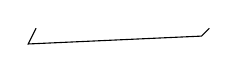
\begin{tikzpicture}\draw (0,0)--(-.1,-.2)--(2.1,-.1)--(2.2,0);\end{tikzpicture}}
}
\figure{\begin{tikzpicture}[x=1cm,y=1cm]\draw (0,0)--(2,-5.4);\draw (-.7,-4)..controls (1,-2.9) and (2.8,-1.2)..(3.7,-.3);\end{tikzpicture}}

Ceci résulte du \uline{lemme}. Pour qu'une \deleted{\unsure{normale}} \inserted{extension} $L$ d'un corps local \deleted{\unsure{abs.}} \unsure{quel} $K$ soit non ramifiée, il faut et il suffit que
\[
N_{L/k}U_L=U_L\unsure{\cap|\parallel}N_{L/k}L^*\supset U_k
\]

\mspage{44}

